% twocurv.tex
% May 2020
% association of follicle curvature and other skin and fleece traits with wrinkle differences in Merinos

\documentclass{article}


% Authors packages
\usepackage{graphicx,lscape,subfigure}
\usepackage{caption,rotating}
\usepackage{tikz}
\usepackage{bm,longtable}
\usepackage{textcomp}
\usepackage{url}


\begin{document}


\title{The two curvatures}
\author{Neville Jackson}
\date{28 June 2020}

\maketitle

\begin{abstract}

Wrinkled Merino sheep usually have a high crimp frequency and highly curved wool follicles and fibres.
We attempt to dissect these associations and show that almost all of them are due to the two factors involved in wrinkle formation, namely presence of hard collagen in the lower dermis, and excessive upper dermal expansion due to the development of secondary follicles.
  We suggest that type and amount of collagen tissue in the lower dermis is a common cause of both follicle curvature and wrinkle. 
  We suggest that a large population of secondary derived follicles is a consequence of all follicles ( including primaries) being small and this in turn leads to small fibres which are intrinsically more curved.
There is published evidence that follicles curve during follicle development and that the presence of hard collagen in the lower dermis at this time interferes with the developing follicle downgrowth causing follicles to grow in a curve.  
 There is also evidence of a strong association between fibre diameter, ortho/para cortical segmentation and general follicle size.

Conventional view of fibre curvature is that it is caused by differences in the ortho and para cortex. It is proposed that this may not be correct, and that both fibre curvature and microstructure difference between ortho and para cortex are caused by the fibre growing inside a curved follicle. 

It is proposed that follicle curvature has two components. Firstly, all follicles in all breeds of sheep are slightly curved and the degree of this component of curvature is related to fibre diameter. Secondly, if a sheep has the type of collagen that is associated with wrinkles, it also has some additional follicle curvature which is caused by collagen interfering with follicle development.

Some data and analyses are presented to support this 'two curvatures' hypothesis.
\end{abstract}


\section{Introduction}

Some time ago there was a wool industry which possessed a reasonable working definition of wool quality that was universally understood among producers, traders, and processors. They even went so far as to put a number on it, and to link it to spinning performance. Quality numbers  or 'Counts' ranged from 100's to 32's , the number referring to the number of hanks of yarn ( each 560 yards long)  which could be spun from 1 pound (0.454Kg) of clean wool, at the spinning limit. The concept is obviously tied to particular processing technologies. What is of interest here is the way quality number was assessed.  It was a visual appraisal of crimp frequency, with a correction for abnormal handle.

Then it was found that fibre fineness ( ie diameter) was a major determinant of spinning performance and softness or handle. There was a period of agonising over the relationship between crimp frequency and fibre diameter. We show some of these investigations in Figure~\ref{fig:crimpdiam} because they are relevant to our current arguments regarding curvature. 
%\documentclass{article}
%\usepackage{graphicx,subfigure}
%\usepackage{caption,rotating}
%\begin{document}

\begin{figure}[]
\centering
 \subfigure[Reviewed by Roberts and Dunlop]{
    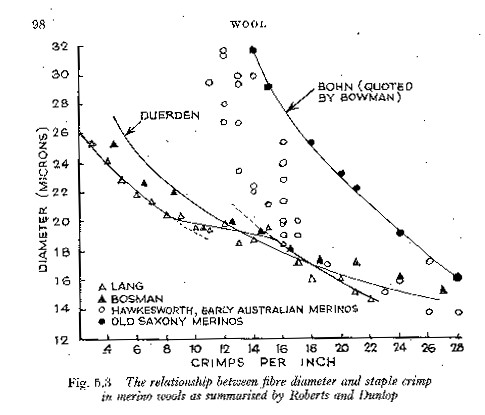
\includegraphics[scale=0.60]{cd1.jpg}
% \includegraphics[width=1.0\textwidth]{w479-2-rigid.jpg}
  }
 \subfigure[Roberts and Dunlop's own data from CSIRO Strain Trial]{
    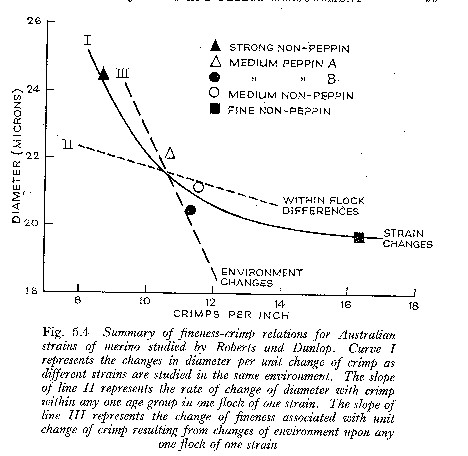
\includegraphics[scale=0.60]{cd2.jpg}
  }
  \caption{Crimp frequency fibre diameter relationships from Roberts and Dunlop(1957)~\cite{robe-1957}. Figures reproduced from Onions(1962)~\cite{onio-1962}}
\vfill
  \label{fig:crimpdiam}
\end{figure}

%\end{document}


Notice that the crimp/diameter relationship is quite steep at low crimp frequencies, but flattens out as one approaches the higher crimp frequencies of fine Merino wools. We are going to argue that the crimp/diameter relationship was historically quite satisfactory for non Merino wools, and that quality numbers as originally used for British sheep breeds were probably an adequate diameter indicator and therefore did indeed  relate to spinning performance. It is the Merino wools for which the quality number system breaks down. We will present new data making this clear; the above published material has an inadequate range, and is just what originally pointed us to the concept of crimp frequency relating to diameter for coarse wools but not for Merino.

Eventually measured fibre diameter replaced subjective quality numbers as a descriptor of wool sold in Australia, and elsewhere. The industry settled down to a period of about 20 years using fibre diameter alone. Then Paul Swan's thesis appeared defining fibre curvature and establishing a basic measurement method for fibre snippets and showing the importance of measurement conditions in ensuring that the fibre was relaxed for measurement (Swan(1993)~\cite{swan-1993}).  Fibre specification eventually became a dual parameter affair, with fibre diameter and fibre curvature both specified, but there is some doubt regarding the validity of the measurement conditions for fibre curvature with both Laserscan and OFDA measurement methods. 

In the middle of these market specification upheavals, sheep breeders also moved from quality numbers to fibre diameter, acknowledging that breeding of fine Merinos towards higher and higher quality numbers had not led to finer fibre diameters. Breeders also became interested, following the work of Nay(1966)~\cite{nay-1966}, in follicle curvature.  Follicle curvature was shown to be genetically correlated with staple crimp frequency, wrinkle score, and bulk compression measurement. The curvature of a follicle was always thought to be the same thing as the intrinsic curvature of a properly relaxed fibre, because it corresponded to the curvature with which the fibre emerged from the follicle. This was never proven. A formula converting follicle curvature scores to intrinsic radius of curvature was established by Jackson and Watts(2016)~\cite{jackson-2016}.

The focus of this document is on what causes follicles and fibres to be curved. There are two schools of thought on causation
\begin{description}
\item[classic view] fibres curve because of their internal structure. In sheep like fine Merinos with a bilateral ortho/para cortical structure, the paracortex is always on the inside of the curve. It is asserted that the paracortex contracts more during keratinization and thus causes the fibre to curve. The follicle passively follows what happens to the fibre. In coarser wooled sheep without bilateral cortical structure this is less clear, but Hynd et al. (2009)~\cite{hynd-2009} assert there is asymmetry in mitotic activity and keratinisation.
\item[follicle view] fibres curve because they form inside a curved follicle. The spatial environment in which the bulb cells differentiate influences their development leading to a different internal structure on the inside and outside of curves and a curved fibre shape.  The observed differences in internal fibre structure are just a side-effect of forming inside a curved follicle, and are not the cause of curvature. To find the cause of fibre curvature we have to look for what causes follicles to curve.  
\end{description}

This document takes the follicle view and attempts to uncover the causes of follicle curvature. It emerges that there is more than one causal factor, and that all are related to skin development, not to fibre structure.

\section{Causation and association}
Everyone u54nderstands that observing a correlation does not prove causation. So what experiments and analyses can one do to establish causation? There are several ways, and we list them
\begin{itemize}
\item Do a designed experiment. If the factors studied are the only difference between treatment groups, and there is proper randomization, then one can conclude the factors are responsible for the differences observed.
\item Establish a time sequence. If A occurs before B, then it is not possible for B to cause A.
\item Find a mechanism. If there is a feasable way in which A could cause B, then it is at least possible for A to cause B. Theories about how things work are very useful here.
\item  Strong correlation. There has to be some association observable between cause and effect. Observing association is a necessary step to establishing a cause, but it is not definitive.
\item Regression with chosen independent X values. This is like a designed factorial experiment. 
\item Repeatability. If a relation is causal it will always be present. 
\item Coherence. If a proposed causal relation fits in with other things known and generally accepted in an area, it is likely to be causal. If it is in disagreement, one has to be careful.
\end{itemize}
 
Behind most of these points is the concept of confounding. Designed experiments attempt to study factors in isolation. In the real world, especially in biology, we are often forced to study traits varying simultaneously.  Causal analysis in this situation  is difficult. One approach is to fit a model corresponding to one's theory of causation and to show that it is a good fit to the data. 


\section{Which comes first follicle or fibre curvature ?}
Evidence on the time sequence of follicle and fibre curvatures is not readily found. There is a photomicrograph in the classic study of Hardy and Lyne (1956)~\cite{hardy-1956} which shows developing follicles in vertical section before the fibre growth has commenced. This photomicrograph is important so we reproduce it here in Figure~\ref{fig:hardylyne}
%\documentclass{article}
%\usepackage{graphicx,subfigure}
%\usepackage{caption,rotating}
%\begin{document}

\begin{figure}[]
\centering
 \subfigure[Plate I from Hardy and Lyne(1956)~\cite{(hardy-1956}]{
  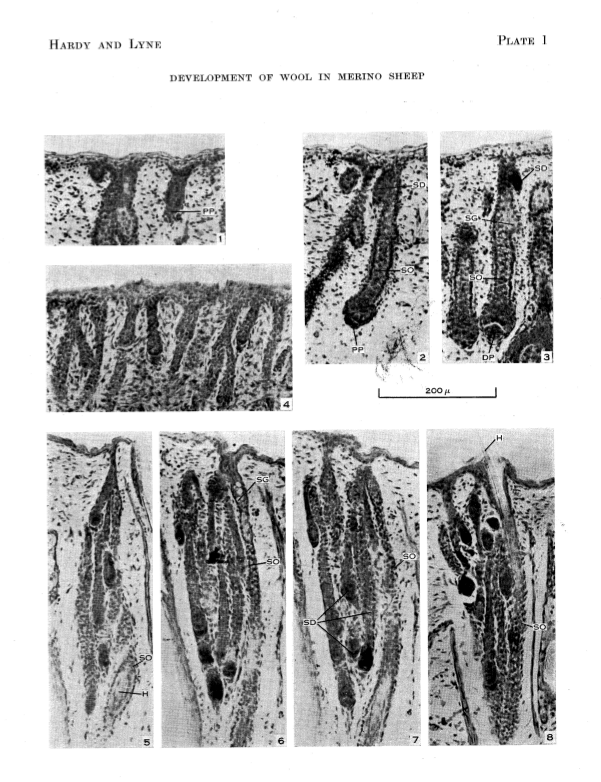
\includegraphics[width=1.0\textwidth]{HardyLyneplate1.png}
  }
 \subfigure[Caption from Hardy and Lyne(1956)~\cite{(hardy-1956}]{
  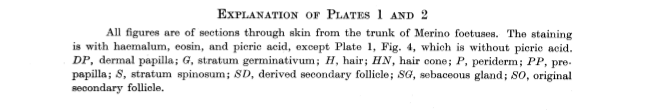
\includegraphics[width=1.0\textwidth]{HardyLynecaption.png}
  }

  \caption{ Follicles at some early stages of development}
\vfill
  \label{fig:hardylyne}
\end{figure}

%\end{document}


The fibre does not start to form before stage F4 and does not emerge from the follicle until stage F8. The first three photomicrographs, ie before stage F4, and the developing follicles show some curvature, especially in the second Figure. The fourth Figure shows branching follicles at day 102 .
This is hardly convincing evidence. The degree of curvature is slight. It is suspected that the Hardy and Lyne used a strong wooled Merino, as this would have been easier material to study vertical sections. 

\section{Follicle curvature and collagen}
As part of a study of association of collagen amount and type with wrinkle, it was observed that sheep in two groups chosen as wrinkle-free or wrinkled differed in amount and type of collagen in the lower dermis (Watts et al. (2020)~\cite{watts-2020}, but also differed in follicle curvature.  The group means for follicle curvature, and for fibre diameter, are shown in Table~\ref{tab:curv}
%\documentclass{article}
%\usepackage{lscape}
%\begin{document}

\begin{table}[htp]
\centering
\caption{Means for follicle curvature, fibre diameter and integrated collagen optical density for wrinkled and wrinkle-free groups of sheep}
\label{tab:curv}
\vspace{0.1in}
\begin{tabular}{|p{2.0in}|p{1.0in}|p{1.0in}|}  \hline
      & Wrinkle-free  &  Wrinkled  \\ 
\hline 
Follicle curvature (score 1-7) & 2.16 & 4.44 \\
Fibre diameter  (micron)    & 17.26 & 18.15 \\
Integrated collagen density (OD) & 280851 & 362991 \\
\hline

\end{tabular}
\end{table}

%\end{document}

The groups were chosen to differ in wrinkle. It has been proposed that the observed collagen difference is the cause of the difference in wrinkle (Watts et al. (2020)~\cite{watts-2020}). We are wondering whether the collagen difference is not also the cause of the difference in follicle curvature. 

What we propose is that presence of hard collagen in foetal skin during follicle development causes developing follicles to bend.  There is visual evidence of this occuring. Dreyer et al. (1983)~\cite{dreyer-1983} published a photomicrograph of Karakul sheep foetal skin in vertical section at 128 days. We reproduce it here in Figure~\ref{fig:dreyer}
%\documentclass{article}
%\usepackage{graphicx,subfigure}
%\usepackage{caption,rotating}
%\begin{document}

\begin{figure}[]
\centering
    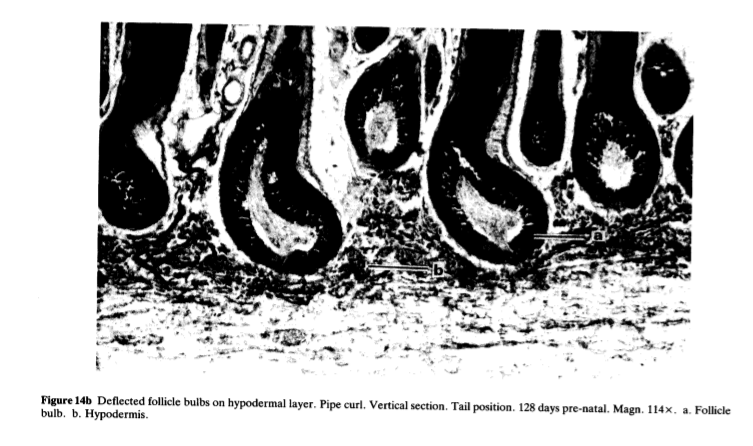
\includegraphics[scale=0.80]{dreyerp6.png}
  \caption{Photomicrograph of foetal skin from Dreyer et al. (1983)~\cite{dreyer-1983} showing follicle bulbs deflecting on contact with the collagen layer. Karakul sheep at 128 days}
\vfill
  \label{fig:dreyer}
\end{figure}

%\end{document}


We quote Dreyer et al
\begin{quote}
"The impression gained was that owing to the vigour of the follicle bulb, the constituent collagen fibres of the hypodermis were displaced in some cases, but no real piercing of that tissue took place. In other cases it would appear theat the follicle bulb and the papilla were undergoing some degree of flattening due to growth pressure on the barrier layer......This barrier effect could also explain the deflection of the bulb to any side as it reacts to the force exerted by downward growth"
\end{quote}
This clearly establishes that the dark stained collagen layer in Figure~\ref{fig:dreyer} acts as a barrier to downward growth of follicles.  If the follicles continue to grow, they must deflect sideways, and this will result in a curved follicle.

\section{Follicle curvature without collagen}
All follicles in non-Merino breeds of sheep have a slight degree of curvature, and their fibres or staples have a range of crimp frequencies less than one up to about 4 crimps per cm.  We may have to exclude Downs wool breeds, here because they have very curved and tangled follicles, and I suspect they have hard collagen induced follicle curvature like Merinos.

We have to consider what causes the curvature of follicles in sheep which do not have hard collagen? The first thing to note is it appears to be quite strongly related to fibre diameter. There are data supporting this in Figure~\ref{fig:crimpdiam} and in the subsection below.

We have to suppose that this is just the inherant asymmetric design of all follicles and that larger follicles with larger fibres are just built to a design with a larger radius of curvature.

\subsection{Data supporting proposal that curvature relates to diameter in non-Merino breeds, but not in Merino}
The breed survey data of Carter(1968)~\cite{carter-1968} offer some support. There are no follicle or fibre curvature measurements, but there is crimp frequency and diameter. So we shall look at the crimp/diameter relationship  across breeds in particular comparing non-Merino with Merino data. Figure~\ref{fig:cartcrimpdia} plots breed means of fibre diameter against crimp frequency
%\documentclass{article}
%\usepackage{graphicx,subfigure}
%\usepackage{caption,rotating}
%\begin{document}

\begin{figure}[]
\centering
    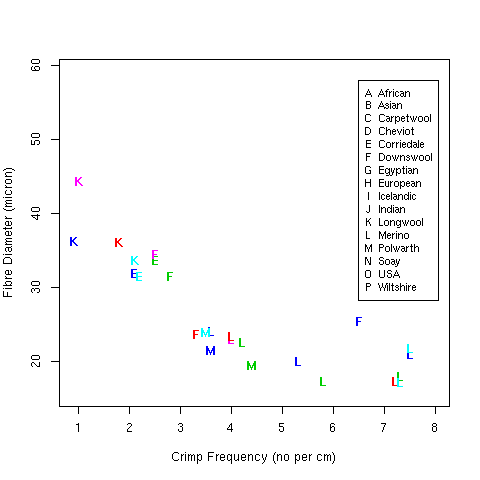
\includegraphics[scale=0.80]{cartercrimpdia.png}
  \caption{Crimp frequency fibre and diameter breed means from Carter(1968)~\cite{carter-1968}. Each point is mean of about 20 sheep from one flock representing a breed.}
\vfill
  \label{fig:cartcrimpdia}
\end{figure}

%\end{document}


There is a clear straight line relationship for crimp frequencies up to about 4 crimps per cm. In the Merino range ( 4 to 8 crimps per cm) there is no relationship at all, and there is one outlier Downs wool breed mean in that range. 

These data have limitations. There are not enough replicate points. We are using crimp frequency as a proxy for follicle curvature. Each point is a mean of about 20 sheep sampled from one flock representing the breed. The only positive is that it extends Figure~\ref{fig:crimpdiam} into the non-Merino breeds.

\section{Can we separate two causes for curvature?}
We are proposing that there is one follicle curvature, that all sheep have, that is related to fibre diameter and follicle size, and that there is a second follicle curvature that only Merinos have, that is caused by  presence of hard Type I collagen in the lower dermis.

Can we separate these {\em two curvatures} by analysing data?  I propose that we can use regression analysis to remove the diameter related part of follicle curvature variation, and then study the remaining variation ans see if it relates to collagen measurements.

\subsection{ Does diameter corrected follicle curvature relate to collagen measurements?}
The only available data that include collagen measurements, follicle curvature and fibre diameter are  from the collagen/wrinkle experiments reported by Watte et al. (2020)~\cite{watts-2020}. Taking all available data from this experiment, we look first at the regression of follicle curvature on mean fibre diameter. This is shown in Figure~\ref{fig:fcd}
%\documentclass{article}
%\usepackage{graphicx,subfigure}
%\usepackage{caption,rotating}
%\begin{document}

\begin{figure}[]
\centering
    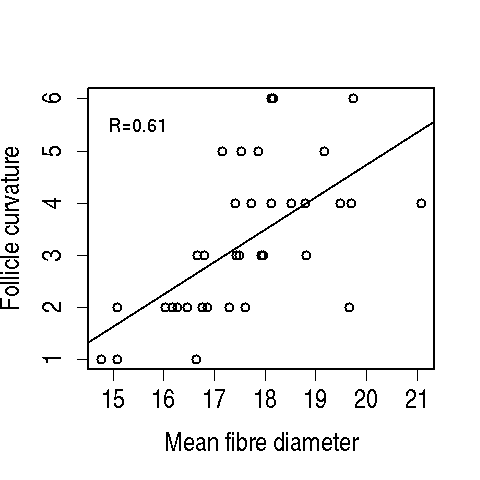
\includegraphics[scale=0.60]{fcd.png}
  \caption{Scatterplot of follicle curvature against mean fibre diameter for 35 sheep in the trial of Watts et al. (2020)~\cite{watts-2020}. Line is the fitted regression $(Fc ~ -7.68 + 0.62 * D)$, and correlation is shown as $R=0.61$.}
\vfill
  \label{fig:fcd}
\end{figure}

%\end{document}


Figure~\ref{fig:fcd} shows all data points, the regression line $(Fc ~  -7.68   + 0.621 * D)$ and the product moment correlation $(0.61)$. So part of the follicle curvature of these sheep is clearly diameter related. 

What we do is remove this diameter related part of follicle curvature by computing the residuals for follicle curvature in Figure~\ref{fig:fcd}. We call these residuals $Fc | D$ (follicle curvature adjusted for diameter) and the computed residuals are shown as a histogram in Figure~\ref{fig:residhist}
%\documentclass{article}
%\usepackage{graphicx,subfigure}
%\usepackage{caption,rotating}
%\begin{document}

\begin{figure}[]
\centering
    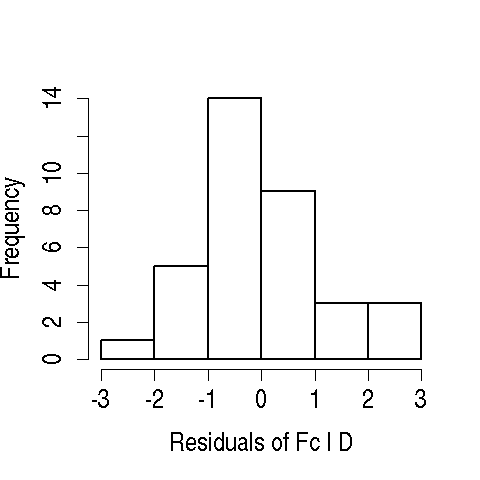
\includegraphics[scale=0.60]{fcdresidhist.png}
  \caption{Histogram histogram of residual variation in follicle curvature after adjusting for regression on mean fibre diameter}
\vfill
  \label{fig:residhist}
\end{figure}

%\end{document}


So this new variable $(Fc | D)$ has nearly as big a range as Fc and has a reasonable normal-looking distribution (this was tested with residual plots).

We can now look to see if this remaining variation in Fc is related to collagen measurements. This relation is shown in Figure~\ref{fig:fcadjdxcoll}
%\documentclass{article}
%\usepackage{graphicx,subfigure}
%\usepackage{caption,rotating}
%\begin{document}

\begin{figure}[]
\centering
    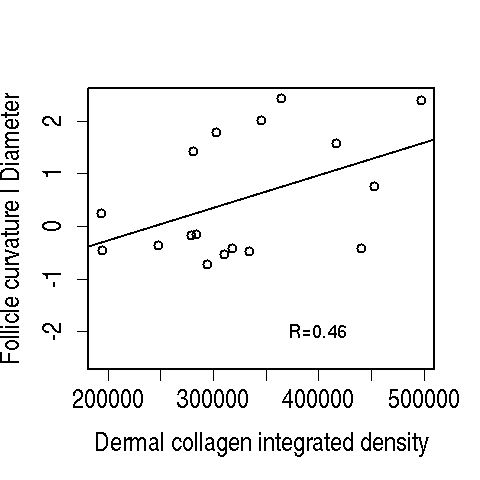
\includegraphics[scale=0.80]{fcadjdcoll.png}
  \caption{Scatterplot of follicle curvature adjusted for diameter against integtated dermal collagen optical density for 17 sheep in the trial of Watts et al. (2020)~\cite{watts-2020}. Line is the fitted regression $(Fc | D ~ -1.49 + 6.17e-06 * Collagen)$, and correlation is shown as $R=0.46$.}
\vfill
  \label{fig:fcadjdxcoll}
\end{figure}

%\end{document}


So Fc adjusted for D does related to collagen. There are only 17 points because this work was incomplete whn Jim Watts passed away. Only 17 sheep had Fc and D and Collagen measurements.

It is worth looking at the residuals from the fit in Figure~\ref{fig:fcadjdxcoll} to see how much variation in Fc still remains, unexplained by either D or Collagen.  We can do this by looking at variances. Variance of Fc was 1.91. Variance of Fc adjusted for D was 1.30. Variance of Fc adjusted for both D and Collagen was 1.04. So we have explained about half the variance of Fc using D and Collagen. The remaining half is probably measurement error, that is errors in scoring Fc and also errors in the D and Collagen measurements used for adjustment.

\subsection{ What else does diameter corrected follicxlce curvature relate to?}

\section{Mechanisms}

------------------------------------------------------------------

This study looks at associations of wrinkle with follicle curvature and other skin and fibre properties. 

\cite{watts-2020} showed that development of skin wrinkle in Merino sheep is associated with two factors
\begin{itemize}
\item presence of hard collagen in the lower dermis 
\item excess growth of the upper dermis relative to that of the subdermis, probably associated with secondary follicle development
\end{itemize}

Therefore, in studying traits associated with wrinkle, one should consider which of the above two factors is contributing to an observed association. Separating a correlation into components in that way is a challenge for experimental design and analysis.  We use .......

----------------------------------------------  -> discussion
Collagen development, secondary follicle development and wrinkle formation  all seem to commence at the same time of approximately 100 days of foetal age.  Follicle initiation ceases at birth ( 150 days) but development of collagen and wrinkles  and maturation of follicles continue into maturity. 
-----------------------------------------------

\section{Materials and Methods}
The experimental design was as reported by ~\cite{watts-2020}i. There were  two experiments. Trial 1 was pairs of wrinkled and wrinkle-free sheep chosen from each of 5 Merino studs. Trial 2 was sets of 9 wrinkled and 9 wrinkle-free sheep chosen from each of 2 commercial Merino flocks.

\subsection{Histological skin processing and observations}

\subsubsection{Vertical skin sections}
Vertical skin sections, approximately 0.3 millimetres wide, were cut freehand with a sharp razor blade on a freezing stage and stained with 0.25 \% Nile blue sulphate, as described by Nay (1973).  The sections were cut parallel with the angle of emergence of fibres to avoid cutting through follicles.

 Mean follicle curvature was scored from 1 = straight follicles to 7 = tangled follicles by reference to a set of standard drawings used by Nay and Johnson (1973).  

The following measurements and scores were available.  All measurements were to an accuracy of $0.02mm$ and were reported in $mm$ units
\begin{description}
\item[Follicle depth] perpendicular distance from skin surface to bottom of follicle bulb (mm)
\item[Follicle straight length(t)] distance from skin surface to bottom of follicle bulb, measured at the angle of the follicle to the surface.(mm)
\item[Follicle sagitta(h)] If the straight follicle length is considered to be the chord of a circle, the sagitta is the height of the arc above the centre of the chord.
\end{description}

From these measurements it was possible to calculate
\begin{description}
\item[Radius of curvature of follicle]  given by $R = h/2 + t^{2}/(8h)$ (mm)
\item[Angle subtended by the arc] given by $\theta = 2 asin(2/(2R))$ (radians)
\item[Follicle curved length] given by $S = R \theta$ (mm)
\end{description}

The measurement of fibre curvature used by the wool industry is the reciprocal of radius of curvature and is in degrees per mm. The reciprocal of our $R$ would be in radians per mm.


\subsubsection{Horizontal skin sections}
Horizontal skin sections were also prepared as described by
Maddocks and Jackson (1988) using frozen section technique and
measurement procedures of Nay (1973). The sections were used to measure
follicle density $(N_{p} + N_{s})$, secondary follicle to primary follicle ratio $(N_{s}/N_{p})$.
 
\subsection{Fibre measurements}
Primary fibre diameter $(D_{p})$ and secondary fibre diameter $(D_{s})$ were measured on horizontal skin sections on a Lanometer at 500x magnification and reported in microns.

\subsection{Macroscopic skin observations}
\subsubsection{Skin sample scores}
In Trial 1 skin observations were conducted on biopsy specimens.
Skin samples were washed in several changes of water, wool stubble trimmed and then examined under a magnifying lamp ( x 3 magnification).  Scores for  suppleness (1 = hardened to 5 = supple) were made. Suppleness is defined as bending easily without deforming. The operator assessed this subjectively by bending the specimen by hand. The operator was blind to the classification of specimens.  A Mitutoyo ballpoint gauge (model no. 2046S) was used to measure compressed thickness of each specimen at four sites .  

\subsubsection{Live sheep scores}
In Trial 2 skin observations were conducted on live sheep at 2 years of age.
Sheep were given visual scores for SkinType. There were two grades, wrinkled and wrinkle-free. In Trial 2 these grades were used to choose extreme sheep for comparative studies. 

\subsection{Statistical Methods}

Data were imported into the R statistical program \cite{rcoreteam-2017} and analysed using the {\em aov()} function for analysis of variance.
Allowance was made for sub-sampling design by choosing  an appropriate error level for F tests in analysis of variance. 

\section{Results}

\subsection{Macro observations on biopsy specimen}
In Table~\ref{tab:macro} we present suppleness scores and percent compressibility of specimens from the sheep from Trial 1.
%\input{tabmacro.tex}
Wrinkled sheep specimens were consistently less supple and less compressible than those of wrinkle-free sheep.
These differences in Suppleness and Compressibility were tested for significance in an analysis of variance shown in Table~\ref{tab:macrot1aov}
%\input{tabmacrot1aov.tex}
The differences between skin types ( wrinkled and wrinkle-free) were significant for both Suppleness and Compressibility. Flock differences were not significant.



\subsection{Follicle characteristics}
A number of follicle attributes seem to differ between wrinkled and wrinkle-free sheep. 

\subsubsection{Follicle curvature scores}
Follicle curvature scores were available for Trial 1. The scores for each sheep are shown on Table~\ref{tab:curv}
%%\documentclass{article}
%\usepackage{lscape}
%\begin{document}

\begin{table}[htp]
\centering
\caption{Means for follicle curvature, fibre diameter and integrated collagen optical density for wrinkled and wrinkle-free groups of sheep}
\label{tab:curv}
\vspace{0.1in}
\begin{tabular}{|p{2.0in}|p{1.0in}|p{1.0in}|}  \hline
      & Wrinkle-free  &  Wrinkled  \\ 
\hline 
Follicle curvature (score 1-7) & 2.16 & 4.44 \\
Fibre diameter  (micron)    & 17.26 & 18.15 \\
Integrated collagen density (OD) & 280851 & 362991 \\
\hline

\end{tabular}
\end{table}

%\end{document}

With exception of Flock 4, the wrinkle-free sheep had a lower follicle curvature score than the wrinkled sheep.

An analysis of variance of these scores is given in Table~\ref{tab:curvaov}
%\input{tabcurvaov.tex}
This shows that the difference between wrinkle-free and wrinkled sheep was significant at the 1 percent level.

\subsubsection{Follicle curvature measurements}
Follicle curvature measurements were made for Trial 2, using methods described in \cite{watts-2018}.  Table~\ref{tab:curvmeasmeans} shows means for follicle depth, straight length of the follicle, curved length of the follicle and radius of curvature. 
%\input{tabcurvmeasmeans.tex}
All four measurements differed between wrinkled and wrinkle-free sheep,and differences were significant for all four traits.  An analysis of follicle curvature measurements is in \cite{watts-2018}. 
The important result is that the wrinkled sheep had a much smaller radius of curvature, meaning that follicles were more curved in wrinkled sheep. This confirms results obtained with subjective follicle curvature scores.  The follicles of wrinkled sheep were also slightly deeper and longer. 

\subsubsection{Follicle density and S/P ratio}
For Trial 2, some further measurements of follicle and fibre characteristics were available, and are shown in Table~\ref{tab:follmeas}
%\input{tabfollmeas.tex}
Wrinkled sheep had lower follicle density, lower S/P ratio, and coarser primary and secondary fibres.  Analyses of variance (Table~\ref{tab:follmeasaov}) confirmed that these differences between wrinkled and wrinkle-free sheep were significant. The Flock differences were not significant.
%\input{tabfollmeasaov.tex}


\section{Discussion}
 
\subsection{Follicle curvature hypothesis}
Perhaps the next most important result is the observation that wrinkled Merinos invariably have curved follicles. We suggest that this happens because down-growth of follicle plugs from the epidermis into the papillary dermis which occurs from days 60-100 in the foetus is interfered with by presence of large amounts of developing collagen in the lower part of the papillary dermis and the reticular dermis. Growth of follicle plugs downward is inhibited by presence of collagen and they continue to grow, but deflect sideways.

There are photomicrographs in \cite{hardy-1956} in which one can actually see follicle plugs curved, before they are growing a fibre. If this is correct we have actually solved the 'chicken and egg' argument about fibre curvature and follicle curvature. Follicle curvature comes first. The fibres curve because they grow into a curved tube. The bilateral ortho and para cortex arrangement in curved Merino fibres is a consequence of the fibre developing in a curved tubular space, not a cause of the curvature. The cortical cells differentiate in a different manner on the inside of the curve, because they are in a more cramped space.

So the spatial distibution of collagen is involved in follicle curvature. That is not quite the same thing as presence of hard collagen, but it suggests that follicle curvature and wrinkle have one common cause.

Apart from being more curved, follicles in wrinkled sheep are also longer. Both straight length and curved length are greater. Also the traditional follicle depth measure, which is average vertical distance of follicle bulbs below the skin surface, is larger in wrinkled sheep.  If presence of collagen makes developing follicles curve, is it possible that it also prolongs their development so that they grow longer? 

There is a biological connection between development of follicles and development of collagen. The papilla cells in follicles are differentiated fibroblasts. The fibrocyte cells which produce collagen fibres are also differentiated fibroblasts.  There is an established theory about the way pre-papilla cells distribute to follicle papillae, and the effects this has on follicle density and fibre diameters \cite{moore-1989,moore-1996}. There is no such theory, that we are aware of, for collagen. It may be that the population of fibroblast cells is limited in number at some stages so that a {\em tradeoff} situation might exist between follicle development and collagen development. This might explain the lower S/P ratio of wrinkled sheep.

\subsection{Predictions and verifications of hypotheses}
We can check if the above hypotheses are robust by using them to predict some previously unobserved phenomena. We make a number of predictions and check each in turn against new data.


\subsubsection{Follicle orientation}
The follicle curvature hypothesis asserts that presence of large amounts of collagen in the developing foetus interferes with down-growth of the follicle plugs causing them to curve. If this is correct one would also expect 
\small
\begin{itemize}
\item[$-$] fibres from such follicles to have more variable emergence angles, 
\item[$-$] the plane of curvature of follicles and fibres to be more variable
\item[$-$] follicle groups to be more disrupted
\end{itemize}
\normalsize
We were not able to check on all of these predictions, but there is a small amount of data shown in Table~\ref{tab:disrupt} comparing wrinkled and wrinkle-free sheep for fibre emergence angle and follicle group orientation.
%\input{tabdisrupt.tex}
The wrinkled sheep are more variable in both fibre emergence angle and follicle group orientation. We have no data on plane of curvature. That would involve looking at orientation of the bilateral ortho/para cortex segmentation.

It seems that follicles in wrinkled sheep are more dislocated, both singly and in groups. That does not prove that foetal collagen development  has caused this.  We can get closer to a verification by plotting amount of collagen ( measured by integrated optical density of PSR stained sections) in adult skin sections against CV of fibre emergence angle for individual sheep. This is done in Figure~\ref{fig:disrupt}
%\input{fig13disrupt.tex}
We see a correlation of 0.47  and a regression line which significant at 1 percent level.  This is not an ideal verification. We really need a study of foetal collagen development against follicle development.

\subsubsection{Curvature and diameter}
Wrinkled sheep have high follicle curvature, but wrinkle-free sheep do not have zero follicle curvature. All sheep (except lustre mutants) have a small degree of follicle curvature, and therefore all wool is crimped. This intrinsic curvature of all follicles has nothing to do with dermal collagen, but seems to be an inbuilt asymmetry in follicles. The interesting thing is that this inbuilt curvature of follicles, and the resultant wavelength of crimp in wool staples, seems to be well related to fibre diameter.  It is the additional curvature which is caused by dermal collagen that is not related to fibre diameter. 

This explains why the traditional method of appraising fibre diameter ( looking at crimp frequency) works quite well for old fashioned coarser wooled sheep, but is not accurate for Merino wool where the presence of collagen and wrinkles adds more curvature and interferes with the relationship with diameter. It also explains why the trend in Australian Fine Merino breeding over the period 1900 to about 1970 towards higher crimp frequencies, did not lead to finer diameters. 
Given the above, we might predict that an analysis of the relationship between crimp ( or follicle curvature) and fibre diameter in Merino sheep should be able to demonstrate that crimp ( or follicle curvature) variation has two parts, one which is diameter related, and one which is wrinkle (or collagen) related.


\subsubsection{Traits correlated with wrinkle score}
Because dermal collagen is a cause of both skin wrinkle and follicle curvature, it would be expected that wrinkle score and follicle curvature score would have a positive genetic correlation. 

There is ample evidence for this. \cite{jackson-1975} obtained a genetic correlation of 0.68 between follicle curvature and wrinkle score.  \cite{jackson-2017a} obtained a genetic correlation of 0.69 with a 95 percent confidence interval of 0.65 to 0.74. Phenotypic and environmental correlations were also positive.

Some slightly more indirect evidence is given by correlations between crimp frequency and wrinkle score. There are other factors in staple crimp apart from follicle curvature, but the relationship is close. One would expect positive correlations between crimp frequency and wrinkle score. 

There are many estimates  of crimp x wrinkle correlation. We take the estimate of \cite{brown-1968} which is $0.28 \pm 0.07$. Not as large, but still positive. Staple crimp is not exactly follicle curvature. 

\subsubsection{Non-Merino breeds}
The two factor wrinkle hypothesis explains why only Merino and Merino derived breeds have skin folds. No other breed has a high S/P ratio , and without this there is insufficient expansionary growth of the dermis and epidermis to cause folding. 

Some non-Merino breeds ( eg Downs wool breeds) have a higher crimp frequency than would be expected for their fibre diameter, and we predict that these breeds  would have a high content of dermal collagen of Type 1.

We do not have the data to check this directly . It is common knowledge that Downs wool has a high fibre curvature but fibre alignment is the staple is very disorganised. This is exactly what one would expect if dermal collagen was interfering with follicle development. It needs to be checked.

Practically nothing is known about breed variation in pin-wrinkle.  We suspect that the Karakul breed may have some form of wrinkle in lambs, but not in adults.   The Karakul does not have a high S/P ratio, but the very curly coat of lambs indicates collagen interfering with follicle development.


\section{Conclusion}


\section*{Acknowledgement(s)}

\bibliographystyle{plain}
\bibliography{twocurv}

\end{document}
